
\documentclass[10pt,oneside,letterpaper,colorhighlight]{book}

\usepackage{alltt}
\usepackage{cite}
\usepackage{plain}
\usepackage{hyperref}
\usepackage{varioref}
\usepackage{array}
\usepackage{xypic}
\usepackage{color}
\usepackage{sectsty}
\usepackage{fancyhdr}
\usepackage{graphics}
\usepackage{fancyvrb}
\usepackage{listings}
\usepackage{makeidx}

\makeindex

\fancypagestyle{plain}{
    \fancyhf{}
    \fancyfoot[C]{\usefont{OT1}{phv}{b}{n}\selectfont \thepage }
    \renewcommand{\footrulewidth}{0pt}
    \renewcommand{\headrulewidth}{0pt}
}

\pagestyle{fancy}

\fancyhf{}
\fancyhead[L]{ \usefont{OT1}{phv}{b}{n}\selectfont \leftmark}
\fancyhead[R]{ \usefont{OT1}{phv}{b}{n}\selectfont \rightmark }
\fancyfoot[C]{\usefont{OT1}{phv}{b}{n}\selectfont \thepage }
\renewcommand{\footrulewidth}{0pt}
\renewcommand{\headrulewidth}{0.5pt}

\renewcommand{\chaptermark}[1]{%
	\markboth{#1}{}}

\renewcommand{\sectionmark}[1]{%
	\markright{#1\ : \thesection}}

\allsectionsfont{\usefont{OT1}{phv}{b}{n}\selectfont}

%%%%%%
%%%%%%

%\renewcommand{\theFancyVerbLine}{\small\textbf{\arabic{FancyVerbLine}}}

\DefineVerbatimEnvironment%
  {xmlCodelisting}{Verbatim}
  {frame=single, 
   framesep=5pt, 
   rulecolor=\color{light}, 
   numbers=left, 
   numbersep=5pt
   commandchars=\\\{\}}

\DefineVerbatimEnvironment%
  {tagExample}{Verbatim}
  {frame=single, 
   framesep=5pt, 
   formatcom=\color{light},
   rulecolor=\color{light},
   commandchars=\\\{\}}

%\lstnewenvironment{xmlCodelisting}%
  %{\lstset{labelstep=1, language=HTML, frame=single, basicstyle=\footnotesize}}
  %{}

%\lstnewenvironment{simpleXmlCodelisting}%
  %{\lstset{labelstep=0, language=HTML, basicstyle=\small}}
  %{}
%
%\lstnewenvironment{javaCodelisting}%
  %{\lstset{labelstep=1, language=Java, frame=single, basicstyle=\footnotesize}}
  %{}


\definecolor{light}{rgb}{0.5,0.5,0.5}

\newenvironment{tagDesc}[1]%
        {
                \begin{center}
                \begin{tabular}{p{0.28\textwidth}cp{0.6\linewidth}}
                \hline 
                \multicolumn{3}{r}{\texttt{<#1>}\hspace{1em}\rule[-0.6em]{0em}{1.7em}}\\
        } {
                \end{tabular}
                \end{center}
        }

\newcommand{\attr}[2] { \texttt{#1} & \vline & {\small#2} \\ \hline }
\newcommand{\childTag}[2] { \texttt{<#1>} & \vline & {\small#2} \\ \hline }
\newcommand{\abstractChildTag}[2] { \textit{\texttt{<ns:#1>}} & \vline & {\small#2} \\ \hline }

\newcommand{\attrs}{
        \hline 
        \textbf{\textsf{Attribute}} & \vline & \textbf{\textsf{Description}}\\ 
        \hline 
}

\newcommand{\noattrs}{
        \multicolumn{3}{c}{\emph{No attributes}}\\
        \hline
}

\newcommand{\tags}{ 
        \\
        \hline
        \textbf{\textsf{Tag}} & \vline & \textbf{\textsf{Description}}\\ 
        \hline 
}


\let\footnoterule\hrule

\newcommand{\indexClass}[1]{\texttt{#1}\index{#1@\texttt{#1} class}}
\newcommand{\class}[1]{\texttt{#1}}

\newcommand{\indexTag}[1]{\texttt{#1}\index{#1@\texttt{#1}}}
\newcommand{\tag}[1]{\texttt{#1}}

\makeatletter
\renewcommand{\@makefntext}[1]%
	{\noindent\makebox[1.8em][r]{\@makefnmark}#1}
\makeatother

\begin{document}

\frontmatter

\begin{titlepage}
\usefont{OT1}{phv}{b}{n}\selectfont
\rule{0pt}{3in}


\noindent
{\Huge Drools Usage Manual}\\
\rule{\textwidth}{1pt}

\vspace{8pt}
\noindent
\usefont{OT1}{phv}{m}{n}\selectfont
{\large version \Large2.0-beta-12}\\
{\small{generated \today}}

\vspace{2in}
\begin{flushright}
\usefont{OT1}{phv}{b}{n}\selectfont
\noindent
{\Large The Drools Project}\\
\rule{2in}{0.5pt}

\vspace{6pt}
{\Large drools.org}
\end{flushright}
\end{titlepage} 

\thispagestyle{empty}
\tableofcontents
\thispagestyle{empty}
\listoffigures
\thispagestyle{empty}

\mainmatter

%
\chapter{Introduction}

\section{Rules}

Many enterprise software systems today already include the concept of
rules.  Most times, these rules are directly implemented in code and
are difficult to adapt to a changing business landscape.  The domain
model many times includes business logic which may change often. When
these business 'rules' are coded using normal systems programming
techniques\footnote{Many times, a long sequence of
\texttt{if}/\texttt{else} statements is used to realize business
rules.}, modification and maintenance of the logic can become
difficult.

Examples of typical simple business rules include:

\begin{itemize}

	\item When a customer applies for a loan of more than \$80,000 
		and has less than \$5,000 in their savings account and
		has had the account for less than 3 years, then reject
		the loan application.

	\item When a customer orders a box of goods and a routed delivery 
		vehicle can include the delivery in today's route by
		lengthening the route by no more than 8 miles, then add
		the customer's delivery to the vehicle.

	\item When a trouble-ticket from a high-priority customer has
		been unresolved for 60 minutes, escalate the urgency of the
		ticket and notify the shift manager.

	\item When a customer buys pie, suggest that they might enjoy
		some ice-cream.
		
\end{itemize}

More complex rules that involve multiple participants or chunks of data
may also exist in systems:

\begin{itemize}

	\item When someone is selling a product desired by another person
		for a price less-than-or-equal-to the price the other is
		is willing to pay, notify both parties.

	\item When an author submits an article and either three junior
		editors a single senior editor has signed off on it, send
		the article to the production department work queue.

	\item When email not directly addressed to me arrives and the
		sender is not on my 'approved' list, then direct it to
		my mail folder that holds potential spam.

\end{itemize}

As companies are often changing the way they do business,  responding
quickly is important.  Changing business logic that
is realized in compiled code can become quite an arduous job.  Systems
that respond to changes in policy and promotions as quickly as 
the enterprise makes decisions reduce maintenance costs and 
development cycle times.


\section{Rules Engines}

Rules engines were created to solve the need for business rules
to be easier to create and maintain. Through the use of intelligent
algorithms (see Chapter \vref{algorithms}), some dedicate rules engine
can also produce efficiencies when working with a great amount of
rules, events and data.

A good rules engine allows the business rules and logic of a system
to be specified external to the system itself.  No longer must these
rules be codified by the developers.  Many rules engines even provide
natural-language or wizard-style GUIs for designing rules, allowing
product managers or business analysts to actually specify the logic.
Separation of concerns and responsibility is achieved by moving the 
business rule specification outside of the actual program logic.
Developers can
concern themselves with systems engineering while the analysts 
concentrate on the business logic.

There are currently many commercial and open-source implementations
of rules engines aside from \drools{}.  The commercial
vendors have undoubtedly good algorithms and have spent considerable
time and effort on the user interfaces and rule specification
languages.

\begin{itemize}
	\item \emph{ILOG JRules}\\
		 \url{http://www.ilog.com/}
	\item \emph{Haley Eclipse}\\
		 \url{http://www.haley.com/}
	\item \emph{Sandia Jess}\\
		 \url{http://herzberg.ca.sandia.gov/jess/}
	\item \emph{CLIPS}\\
		 \url{http://www.ghg.net/clips/CLIPS.html}
\end{itemize}



\section{Standards}

\subsection{RuleML}

RuleML is a mark-up language for describing rules.  After brief
research, we decided that supporting RuleML was not a priority.

\subsection{JSR-94}

JSR-94 is the specification working its way through the Java Community
Process toward defining a common API for rules engines.  This
specification is not yet public, but \drools{} intends to support it 
when it is made available to implementors.



\chapter{Functional Overview}

\section{Rules}

\subsection{Declarative Form}

Drools directly supports \emph{declarative}\index{declarative} rules,
as opposed to \emph{procedural}\index{procedural} logic.  Declarative
rules typically take the form as follows:

\begin{quote}
  \textbf{if} \emph{condition} \\
    \textbf{then} \emph{consequence}
\end{quote}

By ``declarative', it is meant that the rules \emph{declare}, by
way of the \emph{condition}, what should occur but do not specify the
procedure for actually testing the conditions. 
For example, a procedural method for ensuring you have an umbrella if
it is raining would be:

\begin{quote}
    Step outside and determine if it is raining.  If it is raining,
then go to the closet and get an umbrella.
\end{quote}

\noindent
In a declarative form, the above could be represented by two rules:

\begin{itemize}
  \item \textbf{if} \emph{it is raining} \\
    \textbf{then} \emph{you need an umbrella}
  \item \textbf{if} \emph{you need an umbrella} \\
    \textbf{then} \emph{get one from the closet}
\end{itemize}

Given declarative rules, the knowledge that it is raining could
produce two courses of action:

\begin{enumerate}
  \item You already have an umbrella, perhaps because you always carry
one, in which case, you're ready.
  \item You don't have an umbrella, so you go get one from the closet.
\end{enumerate}

\subsection{Applicable Context}

The set of rules to be considered at any point of time depend upon the
current context.  As a human, you have certain rules to think about
when you dine at a fine restaurant, which are exclusive to the set of
rules you consider when spending a sunny day at the swimming pool.
Even so, there are some other overriding rules that may be important
regardless of the context, such as laws against homocide.

So, in a given context, different sets of rules are pertinent.  A
single set of rules may be user in one context, while a different set
is used in a different context. Within a rule-engine, available sets 
of rules are called \emph{rule sets}\index{rule set}.  The set or 
sets of rules currently applicable given the context is called a 
\emph{rule base}\index{rule base}.

\section{Knowledge}

You become aware of knowledge, in the form of facts, over time.
Likewise, over time, facts may change or cease to be true, in 
which case, they facts as you know them must be altered or purged
from your memory.  Likewise, within a rule-engine, there are
operations for becoming aware of a fact, purging a fact, or
modifying a known fact.  These operations are as follow:

\begin{itemize}
  \item \textbf{Assert} Add a fact to what is known.\\
    \emph{The weather is rainy.} \emph{Betty is in the room.}
  \item \textbf{Retract} Remove a fact from what is known.\\
    Removing the fact \emph{Betty is in the room} when Betty leave the
    room.
  \item \textbf{Modify} Alter a fact from what is know.\\
    Changing the knowledge about the weather from \emph{The weather is
    rainy} to \emph{The weather is sunny} when the rain stops and the
    clouds go away.
\end{itemize}

Within a rule-engine, the collected knowledge is called the
\emph{working memory}\index{working memory}.  Knowledge is
asserted, retracted and modified within the working memory and the
rules are evaluated to determine what actions, if any, should be
taken.

\section{Why a rule-engine?}

While the logic expressed in a rule can and has often been writen
within the code a system, a rule-engine offers many benefits.  Instead
of locking the logic up in code written by developers, the logic can
be moved out-board external to the actual application.  In this way
it is possible for non-developers to change the logic without having
to rebuild the system.  Additionally, by codifying all of the system
rules in a central location, they are no longer scattered throughout
the application.  This allows for easier validation of the system's
requirements and analysis of the logic of the system.

Additionally, a rule-engine such as Drools is built upon an
intelligent algorithm that allows for the evaluation of many
rules against many facts in an effecient manner.  In a procedural
system, a change in a single fact might require double-checking
\emph{every} rule to determine if any action needs to be taken.
A rule-engine which uses the \emph{Rete}\index{Rete} algorithm
is optimized to minimize the amount of processing effort that is
required to evaluate the rules that may have been affected by
a change in knowledge.

\section{A note about ``business rules''}

A higher-level form of rule is the \emph{business rule}\index{business
rule}.  Business rules do not necessarily follow the \emph{if-then}
form, but may be specified in different formats that are not as
closely linked to the underlying rule-engine implementation.  Business
rules tend to use the \emph{must} or \emph{must not} form to
expression constraints or inferences.

\begin{itemize}
  \item An order \textbf{must not} be billed before it ships.
  \item An applicant for store credit \textbf{must} be 18 years of age.
\end{itemize}

Drools does not directly support this level of business rules, but
other projects built upon Drools\footnote{The \textbf{Fluxtapose}
suite of tools from The Werken Company is one such product that
supports business rules.} may easily support such
notation.


\chapter{Architecture}

\section{Rules, rule-sets, and rule-bases}

Within Drools, the concepts of rules, rule-sets and rule-bases
are directly modelled by the classes \indexClass{Rule},
\indexClass{RuleSet} and \indexClass{RuleBase}.  A \indexClass{Rule}
may be a member of multiple \indexClass{RuleSet}s, and multiple
\indexClass{RuleSet}s may be active within a given
\indexClass{RuleBase}.

\subsection{\indexClass{Rule}, \indexClass{Condition} and \indexClass{Consequence}}

A single \indexClass{Rule} may have one-or-more
\indexClass{Condition}s associated with it.  Each condition 
must be met before the rule is considered to be activated.
Once activated the rule's \indexClass{Consequence} is a
candidate for being fired.  In pattern parlance, the
\indexClass{Condition} class is simply a \emph{predicate
object}\index{predicate object} which evaluates itself against
the known facts to return a boolean value of either \emph{true}
or \emph{false}.  The \indexClass{Consequence} class is likewise
simply a \emph{functor} which objectifies a function and performs
an arbitrary task when executed.

\begin{figure}[h]
  \begin{center}
  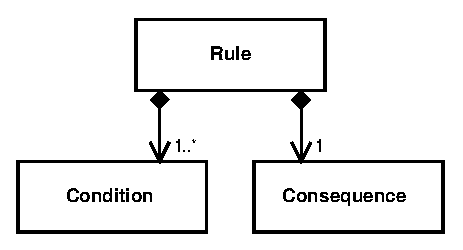
\includegraphics{rule}
  \end{center}
  \caption{Object model for \class{Rule}, \class{Condition} and \class{Consequence}}
\end{figure}

\subsection{\indexClass{RuleSet}}

A \indexClass{RuleSet} is simply a collection of \indexClass{Rule}s.
It serves only to associate a group of rules with one another so that
they may be worked with as a set.

\begin{figure}
  \begin{center}
  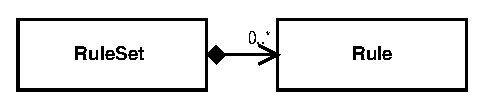
\includegraphics{ruleset}
  \end{center}
  \caption{Object model for \class{RuleSet} and \class{Rule}}
\end{figure}

\subsection{\indexClass{RuleBase}}

A \indexClass{RuleBase} is an \emph{active} collection of
\indexClass{RuleSet}s.  A \indexClass{RuleBase} contains rules
that are all considered to be in effect for a given set of
knowledge.  Multiple \class{RuleSet}s may be a part of a 
given \class{RuleBase}.

\begin{figure}
  \begin{center}
  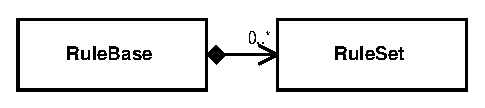
\includegraphics{rulebase}
  \end{center}
  \caption{Object model for \class{RuleBase} and \class{RuleSet}}
\end{figure}

\section{Knowledge}

The set of knowledge that is examined is modelled by the class
\indexClass{WorkingMemory}, which is backed by a particular
\indexClass{RuleBase}.  It is through the \indexClass{WorkingMemory}
that knowledge is \emph{asserted}, \emph{retracted} and
\emph{modified}.
Each \class{WorkingMemory} is backed by exactly one
\indexClass{RuleBase} which determines which rules are evaluated
as knowledge is manipulated.

\begin{figure}
  \begin{center}
  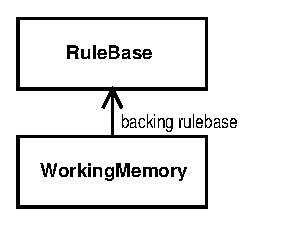
\includegraphics{workingmemory}
  \end{center}
  \caption{Object model for \class{WorkingMemory} and \class{RuleBase}}
\end{figure}

\clearpage

\section{Complete Model}

\begin{figure}[h]
  \begin{center}
  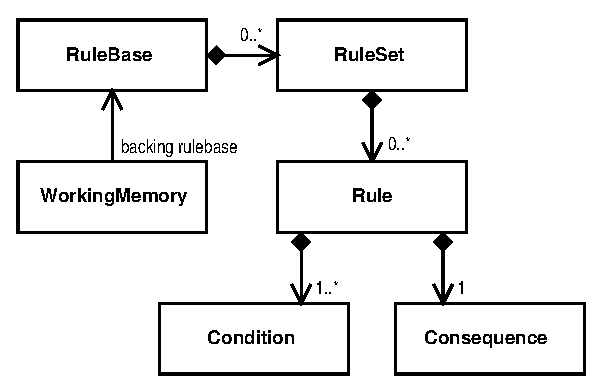
\includegraphics{architecture}
  \end{center}
  \caption{Complete object model}
\end{figure}

\chapter{Drools Rule Langauge}

\section{Introduction}

\drools{} defines a semantic-module-independant rule language created 
called the \emph{Drools Rule Language}.  DRL is a an XML-based
language that uses modern XML features such as XML-Namespaces and XML
Schema. The DRL engine within \drools{} is built on top of
jakarta-commons-jelly, which is a general XML tag library
engine. 

\section{DRL Files}

DRL files are XML files using the DRL tags. They are typically files
that have the \emph{.drl} suffix.  \drools{} only requires that they
be accessible through a URL:

\begin{itemize}
	\item \textbf{\textsf{Local Filesystem}} \\
		DRL files can be stored in the local filesystem and
		accessed using \verb|file://| URLs.
	\item \textbf{\textsf{Web/FTP Server}} \\
		DRL files can be stored on the network and
		accessed using \verb|http://| and \verb|ftp://| URLs.
	\item \textbf{\textsf{Java Classpath}} \\
		DRL files can be stored in the Java classpath or in a JAR
		file, and accessed using the \verb|getResource()| method
		on \verb|java.lang.ClassLoader| and \verb|java.lang.Class|
		classes.
\end{itemize}

\section{Loading DRL Files}

A \verb|RuleSetLoader| is provided for loading DRL files into a
\verb|RuleBase|.  Given a URL, the \verb|RuleSetLoader| will retrieve
the DRL file and load all rules and rule-sets into the specified
\verb|RuleBase| which can then immediately be use for knowledge
manipulation.

\begin{codelisting}
import org.drools.RuleBase;
import org.drools.WorkingMemory;
import org.drools.io.RuleSetLoader;
...

    RuleBase ruleBase = new RuleBase();

    RuleSetLoader loader = new RuleSetLoader();

    loader.load( rulesUrl, ruleBase );

    WorkingMemory memory = ruleBase.createWorkingMemory();

    memory.assertObject( account );
\end{codelisting}

\section{Base DRL Syntax}

The base syntax for DRL contains a small handful of tags 
representing the general structure of rules and rule-sets.
These tags are defined for the XML namespace URI of
\verb|http://drools.org/rules|.

\begin{itemize}
	\item \verb|<rules>|\\
		General outter-level wrapper tag.
	\item \verb|<rule-set>|\\
		A named collection of rules.
	\item \verb|<rule>|\\
		A single rule.
	\item \verb|<parameter>|\\
		A root fact-object parameter.
	\item \verb|<declaration>|\\
		A local variable declaration.
	\item \verb|<extraction>|\\
		A fact extraction.
	\item \verb|<condition>|\\
		A filtering condition.
	\item \verb|<duration>|\\
		The match duration.
	\item \verb|<consequence>|\\
		The rule match consequence.
	\item \verb|<semantics>|\\
		Load a semantic module.
\end{itemize}

\subsection{\texttt{drl:rules}}

The outtermost tag in each DRL file is the \verb|<rules>| tag.  It has
no attributes and serves only to aggregate \verb|<rule-set>|s and
\verb|<rule>|s. The XML namespace declaration for the base DRL should
be affixed to this element.

\begin{codelisting}
<rules xmlns:drl="http://drools.org/rules">
\textcolor{light}{  <drl:rule-set ...>
    ...
  </drl:rule-set>
  <drl:rule ...>
    ...
  </drl:rule>}
</drl:rules>
\end{codelisting}

\subsection{\texttt{drl:rule-set}}

The \verb|<rule-set>| is a named container for \verb|<rules>|.  Its
only attribute is \verb|name| to provide for a name.  

\begin{codelisting}
<drl:rule-set name="Gold-Level Member Rules">
\textcolor{light}{  <drl:rule ...>
    ...
  </drl:rule>}
</drl:rule-set>
\end{codelisting}

\subsection{\texttt{drl:rule}}

The \verb|<rule>| tag is the most complex.  It \emph{must} contain
at least one \verb|<parameter>| and a \verb|<consequence>| tag.  It
may optionally contain \verb|<declaration>|, \verb|<extraction>|,
\verb|<condition>| and \verb|<duration>| tags.  The \verb|name|
attribute must be present. A \verb|<rule>| may exist inside either 
a \verb|<rules>| or \verb|<rule-set>| tag.

\begin{codelisting}
<drl:rule name="Over Credit Limit">
\textcolor{light}{  <drl:parameter ..>
    ...
  </drl:parameter>
  <drl:declaration ..>
    ...
  </drl:declaration>
  <drl:extraction ..>
    ...
  </drl:extraction>
  <drl:condition ..>
    ...
  </drl:condition>
  <drl:duration ..>
    ...
  </drl:duration>
  <drl:consequence ..>
    ...
  </drl:consequence>}
</drl:rule>
\end{codelisting}

\subsection{\texttt{drl:parameter}}

The \verb|<parameter>| tag defines a root fact object that the
rule expects to be provided from external resources.  The only
attribute is \verb|identifier| which provides the variable identifier
to be used to refer to the object elsewhere in the rule. The content
of the tag is dependent upon the semantic module used for the rule.
For illustration purposes, the Java Semantic Module has been used.

\begin{codelisting}
<parameter identifier="customer">
\textcolor{light}{  <java:class type="com.werken.Customer"/>}
</parameter>
<parameter identifier="account">
\textcolor{light}{  <java:class type="com.werken.Account"/>}
</parameter>
\end{codelisting}

\subsection{\texttt{drl:declaration}}

A \verb|<declaration>| tag is similar to a \verb|<parameter>| in
that it defines a typed and named object.  It must contain an
\verb|identifier| attribute to specify the name that may be used
to refer to the declared object elsewhere in the rule.  This tag
declares a variable that must be populated internally using an
\verb|<extraction>|.  For illustration purposes, the Java Semantic
Module has been used.

\begin{codelisting}
<drl:declaration identifier="custName">
\textcolor{light}{  <java:class type="java.lang.String"/>}
</drl:declaration>
<drl:declaration identifier="acctBalance">
\textcolor{light}{  <java:class type="java.math.BigInteger"/>}
</drl:declaration>
\end{codelisting}

\subsection{\texttt{drl:extraction}}

An \verb|<extraction>| defines a fact extraction.  Its only
attribute is \verb|target| which names the parameter or declaration
that the extracted fact should be assigned to.  The content
of the tag is dependent upon the semantic module used for the rule.
For illustration purposes, the Java Semantic Module has been used.

\begin{codelisting}
<drl:extraction target="customer">
\textcolor{light}{  <java:extractor>account.getCustomer()</java:extractor>}
</drl:extraction>
<drl:extraction target="custName">
\textcolor{light}{  <java:extractor>customer.getName()</java:extractor>} 
</drl:extraction>
<drl:extraction target="acctBalance">
\textcolor{light}{  <java:extractor>account.getBalance()</java:extractor>}
</drl:extraction>
\end{codelisting}

\subsection{\texttt{drl:condition}}

The \verb|<condition>| defines a condition that must be met in
order for the rule to match. It contains the main logic of the rule.
The content of the tag is dependent upon the semantic module used for the rule.
For illustration purposes, the Java Semantic Module has been used.

\begin{codelisting}
<drl:condition>
\textcolor{light}{  <java:condition>custName.equals( "McWhirter" )</java:condition>}
</drl:condition>
<drl:condition>
\textcolor{light}{  <java:condition>acctBalance.signum() == 0</java:condition>}
</drl:condition>>
\end{codelisting}

\subsection{\texttt{drl:duration}}

The \verb|<duration>| tag is used to specify a temporal condition.
The truth duration of a rule is the amount of time that all other
conditions must hold true before a match is determined.  The
content of the tag is dependent upon the semantic module used
for the rule. A simple \verb|<fixed-duration>| tag is supplied as
part of the base DRL syntax in order to specify static durations
that are not dependent upon rule data.

\begin{codelisting}
<drl:duration>
  <drl:fixed-duration seconds=".."
                      minutes=".."
                      hours=".."
                      days=".."
                      weeks=".."/>
</drl:duration>
\end{codelisting}

\subsection{\texttt{drl:consequence}}

The \verb|<consequence>| tag defines the action to be taken
once a rule matches for a set of root fact objects.  The content
of the tag is dependent upon the semantic module used for the rule.
For illustration purposes, the Java Semantic Module has been used.

\begin{codelisting}
<drl:consequence>
\textcolor{light}{  <java:consequence>
    account.addMoney( new BigInteger( "1000000" ) );
  </java:consequence>}
</drl:consequence>
\end{codelisting}


\subsection{\texttt{drl:semantics}}

The \verb|<semantics>| tag is used to load a semantic module.
It has no content and the \verb|module| attribute is required
in order to identify a semantic module to load.

\begin{codelisting}
<drl:semantics module="org.drools.semantics.java"/>
\end{codelisting}


%\chapter{Usage}

\section{\drools{} Client API}

\subsection{Introduction}

\drools{} is divided into several sets of APIs.  The core client API
is by far the simplest and most commonly used by developers.  The
core \drools{} client API consists of locating a rule-base, creating
a working memory, and then managing fact assertion, modification and
retraction.

\subsection{Locating a Rule-base}

\verb|RuleBase| objects are typically loaded from a
\verb|RuleBaseRepository|.  Different repository implementations
provide different mechanisms for the storage of each
\verb|RuleBase|.  The method by which your project obtains
a \verb|RuleBaseRepository| is implementation-specific but
may involve a lookup and discovery mechanism such as JNDI.

Once a \verb|RuleBaseRepository| has been obtained, the
simple method\\ \verb|lookupRuleBase(..)| method is used
to retrieve a \verb|RuleBase| by its URI.\footnote{URIs that
identify rule bases are not necessarily deferenceable.  They
serve only as unique identifiers for a collection of rules.}

\bigskip
\begin{codelisting}
RuleBaseRepository repo = myUtilities.getRepository();

String ruleBaseUri = "http://rules.werken.com/family-relationships";

RuleBase ruleBase = repo.lookupRuleBase( ruleBaseUri );
\end{codelisting}

\newpage

\subsection{Creating a Working Memory}

\drools{} provides two different types of working memory
implementations: a normal \verb|WorkingMemory| and a
\verb|TransactionWorkingMemory|.

\begin{itemize}

	\item \textbf{\textsf{WorkingMemory}} \\
		The normal \verb|WorkingMemory| implementation 
		propagates fact assertions, modifications and
		retractions through the Rete-OO network in
		real-time.  Once the fact manipulation 
		methods return control to the client program,
		all facts have been assimilated and acted upon.

	\item \textbf{\textsf{TransactionalWorkingMemory}} \\
		The \verb|TransactionalWorkingMemory| does \emph{not}
		propagate fact manipulation information through the
		Rete-OO in real-time.  Instead, it calculates the net
		fact changes and performs all manipulations immediately
		upon usage of the \verb|commit()| method.  No actions
		are performed until \verb|commit()| is called, and
		all fact information is discarded if \verb|abort()|
		is used.

\end{itemize}

The methods on \verb|RuleBase| to construct working memories are:

\bigskip

\begin{codelisting}    
/** Create a WorkingMemory session for this RuleBase.
 *
 *  @see WorkingMemory
 *
 *  @return A newly initialized WorkingMemory.
 */
public WorkingMemory createWorkingMemory() 

/** Create a TransactionalWorkingMemory session for this RuleBase.
 *
 *  @see TransactionalWorkingMemory
 *
 *  @return A newly initialized TransactionalWorkingMemory.
 */
public TransactionalWorkingMemory createTransactionalWorkingMemory()
\end{codelisting}

\subsection{Fact Manipulation}

Once you have a \verb|WorkingMemory| in hand, you must assert fact
objects to make them available to \drools{} for analysis.  Additionally, as facts
change, the engine must be notified.  Likewise, when an object should
no longer be considered for analysis, it must be retracted from
the engine.  Methods for these three actions are defined upon the
\verb|WorkingMemory| class.

\bigskip

\footnotesize
\begin{alltt}
/** Assert a new fact object into this working memory.
*
*  @param object The object to assert.
*
*  @throws AssertionException if an error occurs during assertion.
*/
public void assertObject(Object object) throws AssertionException
\newpage
/** Modify a fact object in this working memory.
*
*  With the exception of time-based nodes, modification of
*  a fact object is semantically equivalent to retracting and
*  re-asserting it.
*
*  @param object The object to modify.
*
*  @throws FactException if an error occurs during modification.
*/
public void modifyObject(Object object) throws FactException

/** Retract a fact object from this working memory.
*
*  @param object The object to retract.
*
*  @throws RetractionException if an error occurs during retraction.
*/
public void retractObject(Object object) throws RetractionException
\end{alltt}
\normalsize

\section{JSR-94 API}

The \drools{} project is currently working on a JSR-94 API binding.


%\chapter{Drools Rule Langauge}

\section{Introduction}

\drools{} defines a semantic-module-independant rule language created 
called the \emph{Drools Rule Language}.  DRL is a an XML-based
language that uses modern XML features such as XML-Namespaces and XML
Schema. The DRL engine within \drools{} is built on top of
jakarta-commons-jelly, which is a general XML tag library
engine. 

\section{DRL Files}

DRL files are XML files using the DRL tags. They are typically files
that have the \emph{.drl} suffix.  \drools{} only requires that they
be accessible through a URL:

\begin{itemize}
	\item \textbf{\textsf{Local Filesystem}} \\
		DRL files can be stored in the local filesystem and
		accessed using \verb|file://| URLs.
	\item \textbf{\textsf{Web/FTP Server}} \\
		DRL files can be stored on the network and
		accessed using \verb|http://| and \verb|ftp://| URLs.
	\item \textbf{\textsf{Java Classpath}} \\
		DRL files can be stored in the Java classpath or in a JAR
		file, and accessed using the \verb|getResource()| method
		on \verb|java.lang.ClassLoader| and \verb|java.lang.Class|
		classes.
\end{itemize}

\section{Loading DRL Files}

A \verb|RuleSetLoader| is provided for loading DRL files into a
\verb|RuleBase|.  Given a URL, the \verb|RuleSetLoader| will retrieve
the DRL file and load all rules and rule-sets into the specified
\verb|RuleBase| which can then immediately be use for knowledge
manipulation.

\begin{codelisting}
import org.drools.RuleBase;
import org.drools.WorkingMemory;
import org.drools.io.RuleSetLoader;
...

    RuleBase ruleBase = new RuleBase();

    RuleSetLoader loader = new RuleSetLoader();

    loader.load( rulesUrl, ruleBase );

    WorkingMemory memory = ruleBase.createWorkingMemory();

    memory.assertObject( account );
\end{codelisting}

\section{Base DRL Syntax}

The base syntax for DRL contains a small handful of tags 
representing the general structure of rules and rule-sets.
These tags are defined for the XML namespace URI of
\verb|http://drools.org/rules|.

\begin{itemize}
	\item \verb|<rules>|\\
		General outter-level wrapper tag.
	\item \verb|<rule-set>|\\
		A named collection of rules.
	\item \verb|<rule>|\\
		A single rule.
	\item \verb|<parameter>|\\
		A root fact-object parameter.
	\item \verb|<declaration>|\\
		A local variable declaration.
	\item \verb|<extraction>|\\
		A fact extraction.
	\item \verb|<condition>|\\
		A filtering condition.
	\item \verb|<duration>|\\
		The match duration.
	\item \verb|<consequence>|\\
		The rule match consequence.
	\item \verb|<semantics>|\\
		Load a semantic module.
\end{itemize}

\subsection{\texttt{drl:rules}}

The outtermost tag in each DRL file is the \verb|<rules>| tag.  It has
no attributes and serves only to aggregate \verb|<rule-set>|s and
\verb|<rule>|s. The XML namespace declaration for the base DRL should
be affixed to this element.

\begin{codelisting}
<rules xmlns:drl="http://drools.org/rules">
\textcolor{light}{  <drl:rule-set ...>
    ...
  </drl:rule-set>
  <drl:rule ...>
    ...
  </drl:rule>}
</drl:rules>
\end{codelisting}

\subsection{\texttt{drl:rule-set}}

The \verb|<rule-set>| is a named container for \verb|<rules>|.  Its
only attribute is \verb|name| to provide for a name.  

\begin{codelisting}
<drl:rule-set name="Gold-Level Member Rules">
\textcolor{light}{  <drl:rule ...>
    ...
  </drl:rule>}
</drl:rule-set>
\end{codelisting}

\subsection{\texttt{drl:rule}}

The \verb|<rule>| tag is the most complex.  It \emph{must} contain
at least one \verb|<parameter>| and a \verb|<consequence>| tag.  It
may optionally contain \verb|<declaration>|, \verb|<extraction>|,
\verb|<condition>| and \verb|<duration>| tags.  The \verb|name|
attribute must be present. A \verb|<rule>| may exist inside either 
a \verb|<rules>| or \verb|<rule-set>| tag.

\begin{codelisting}
<drl:rule name="Over Credit Limit">
\textcolor{light}{  <drl:parameter ..>
    ...
  </drl:parameter>
  <drl:declaration ..>
    ...
  </drl:declaration>
  <drl:extraction ..>
    ...
  </drl:extraction>
  <drl:condition ..>
    ...
  </drl:condition>
  <drl:duration ..>
    ...
  </drl:duration>
  <drl:consequence ..>
    ...
  </drl:consequence>}
</drl:rule>
\end{codelisting}

\subsection{\texttt{drl:parameter}}

The \verb|<parameter>| tag defines a root fact object that the
rule expects to be provided from external resources.  The only
attribute is \verb|identifier| which provides the variable identifier
to be used to refer to the object elsewhere in the rule. The content
of the tag is dependent upon the semantic module used for the rule.
For illustration purposes, the Java Semantic Module has been used.

\begin{codelisting}
<parameter identifier="customer">
\textcolor{light}{  <java:class type="com.werken.Customer"/>}
</parameter>
<parameter identifier="account">
\textcolor{light}{  <java:class type="com.werken.Account"/>}
</parameter>
\end{codelisting}

\subsection{\texttt{drl:declaration}}

A \verb|<declaration>| tag is similar to a \verb|<parameter>| in
that it defines a typed and named object.  It must contain an
\verb|identifier| attribute to specify the name that may be used
to refer to the declared object elsewhere in the rule.  This tag
declares a variable that must be populated internally using an
\verb|<extraction>|.  For illustration purposes, the Java Semantic
Module has been used.

\begin{codelisting}
<drl:declaration identifier="custName">
\textcolor{light}{  <java:class type="java.lang.String"/>}
</drl:declaration>
<drl:declaration identifier="acctBalance">
\textcolor{light}{  <java:class type="java.math.BigInteger"/>}
</drl:declaration>
\end{codelisting}

\subsection{\texttt{drl:extraction}}

An \verb|<extraction>| defines a fact extraction.  Its only
attribute is \verb|target| which names the parameter or declaration
that the extracted fact should be assigned to.  The content
of the tag is dependent upon the semantic module used for the rule.
For illustration purposes, the Java Semantic Module has been used.

\begin{codelisting}
<drl:extraction target="customer">
\textcolor{light}{  <java:extractor>account.getCustomer()</java:extractor>}
</drl:extraction>
<drl:extraction target="custName">
\textcolor{light}{  <java:extractor>customer.getName()</java:extractor>} 
</drl:extraction>
<drl:extraction target="acctBalance">
\textcolor{light}{  <java:extractor>account.getBalance()</java:extractor>}
</drl:extraction>
\end{codelisting}

\subsection{\texttt{drl:condition}}

The \verb|<condition>| defines a condition that must be met in
order for the rule to match. It contains the main logic of the rule.
The content of the tag is dependent upon the semantic module used for the rule.
For illustration purposes, the Java Semantic Module has been used.

\begin{codelisting}
<drl:condition>
\textcolor{light}{  <java:condition>custName.equals( "McWhirter" )</java:condition>}
</drl:condition>
<drl:condition>
\textcolor{light}{  <java:condition>acctBalance.signum() == 0</java:condition>}
</drl:condition>>
\end{codelisting}

\subsection{\texttt{drl:duration}}

The \verb|<duration>| tag is used to specify a temporal condition.
The truth duration of a rule is the amount of time that all other
conditions must hold true before a match is determined.  The
content of the tag is dependent upon the semantic module used
for the rule. A simple \verb|<fixed-duration>| tag is supplied as
part of the base DRL syntax in order to specify static durations
that are not dependent upon rule data.

\begin{codelisting}
<drl:duration>
  <drl:fixed-duration seconds=".."
                      minutes=".."
                      hours=".."
                      days=".."
                      weeks=".."/>
</drl:duration>
\end{codelisting}

\subsection{\texttt{drl:consequence}}

The \verb|<consequence>| tag defines the action to be taken
once a rule matches for a set of root fact objects.  The content
of the tag is dependent upon the semantic module used for the rule.
For illustration purposes, the Java Semantic Module has been used.

\begin{codelisting}
<drl:consequence>
\textcolor{light}{  <java:consequence>
    account.addMoney( new BigInteger( "1000000" ) );
  </java:consequence>}
</drl:consequence>
\end{codelisting}


\subsection{\texttt{drl:semantics}}

The \verb|<semantics>| tag is used to load a semantic module.
It has no content and the \verb|module| attribute is required
in order to identify a semantic module to load.

\begin{codelisting}
<drl:semantics module="org.drools.semantics.java"/>
\end{codelisting}

%\chapter{Semantic Modules}

\chapter{Java Semantic Module}

\section{Overview}

The Java Semantic Module provides implementations of semantic
components that adhere to the Java language semantics.  The components
can be used directoy from Java with through a DRL file.


\begin{itemize}
	\item \textbf{\textsf{org.drools.semantics.java.ClassObjectType}}\\
		A \verb|ObjectType| implementation that adheres
		to Java class types.  Usable within \verb|<parameter>|
		and \verb|<declaration>| DRL tags.
	\item \textbf{\textsf{org.drools.semantics.java.ExprCondition}}\\
		A \verb|Condition| implementation that uses boolean
		Java expressions for filtering. Usable within 
		\verb|<condition>| DRL tags.
	\item \textbf{\textsf{org.drools.semantics.java.ExprExtractor}}\\
		A \verb|Extractor| implementation that uses Java
		expressions for extracting new facts.  Usable
		within \verb|<extraction>| DRL tags.
	\item \textbf{\textsf{org.drools.semantics.java.BlockConsequence}}\\
		A \verb|Consequence| impementation that uses
		A block of Java statements as the action of a
		matched rule.  Usable within \verb|<consequence>|
		DRL tags.
\end{itemize}

\clearpage

\section{Usage with DRL}

\subsection{Loading the Module}

The Java Semantic Module's tags exist within the XML namespace
URI of \verb|http://drools.org/semantics/java| and within the
Java package of\\ \verb|org.drools.semantics.java|.  To use the
Java Semantic Module within a DRL file, the DRL \verb|<semantics>|
tag must be used, as must an XML namespace prefix binding.

\begin{codelisting}
\textcolor{light}{<drl:rules xmlns:drl="http://drools.org/rules"}
       xmlns:java="http://drools.org/semantics/java"\textcolor{light}{>}

  <drl:semantics module="org.drools.semantics.java"/>

  \textcolor{light}{<drl:rule ...>
    <drl:parameter identifier="account">}
      <java:class type="com.werken.Account"/>
    \textcolor{light}{</drl:parameter>
  </drl:rule>

</drl:rules>}
\end{codelisting}


\subsection{\texttt{java:class}}

The \verb|<java:class>| tag defines an \emph{object type} that adheres
to Java class semantics for types.  It has a single attribute of
\verb|type| which takes a class name as a value.  The tag may be
used as the content of both \verb|<drl:parameter>| and
\verb|<drl:declaration>| DRL tags.

\begin{codelisting}
\textcolor{light}{<drl:parameter identifier="account">}
  <java:class type="com.werken.Account"/>
\textcolor{light}{</drl:parameter>
<drl:declaration identifier="person">}
  <java:class type="com.werken.Person"/>
\textcolor{light}{</drl:declaration>}
\end{codelisting}

\subsection{\texttt{java:condition}}

The \verb|<java:condition>| tag defines an \emph{condition} that
adheres to Java boolean expression semantics.  It has no
attributes and the body content is the boolean expression to
evaluate.  The tag may be used as the content of a \verb|<drl:condition>|
tag.

\begin{codelisting}
\textcolor{light}{<drl:condition>}
  <java:condition>acctBalance == 0</java:condition>
\textcolor{light}{</drl:condition>}
\end{codelisting}

\subsection{\texttt{java:extractor}}

The \verb|java:extractor| tags defines a \emph{fact extractor}
that adheres to Java expression semantics.  It has
no attributes and the body content is the expression to generate
the new fact.  The tag may be used as the content of a 
\verb|<drl:extraction>| tag.

\begin{codelisting}
\textcolor{light}{<drl:extraction target="accountBalance">}
  <java:extractor>person.getAccount().getBalance()</java:extractor>
\textcolor{light}{</drl:extraction>}
\end{codelisting}

\subsection{\texttt{java:consequence}}

The \verb|<java:consequence>| tag defines a \emph{rule consequence}
that adheres to Java statement block semantics.  It may exist as the
content of a \verb|<drl:consequence>| tag.  It has no
attributes and the body content is the set of statements
to execute upon rule match.


\begin{codelisting}
\textcolor{light}{<drl:consequence>}
   System.err.println( "The balance is: " + acctBalance );
   theRepoMan.addAccount( account );
   assertObject( theRepoMan );
\textcolor{light}{</drl:consequence>}
\end{codelisting}


\chapter{XML Semantic Module}

\dots not implemented yet \dots


%
\chapter{Rule Assembly}

\section{Overview}

Only a handful of classes are required to assemble rules once a
\emph{semantic module} has been selected.  Each rule is codified as an
instance of the \verb|Rule| class which may be a member of a
\verb|RuleSet| collection.  

\begin{enumerate}
	\item Instantiate a \verb|Rule|.
	\item Add a \verb|Declaration| for each root fact object.
	\item Add a \verb|FactExtraction| for each fact extraction.
	\item Add a \verb|Condition| for each restrictive condition.
	\item Add a \verb|Consequence| for performing the result of a match.
	\item Add the \verb|Rule| to a \verb|RuleBase|.
	\item Optionally register the \verb|RuleBase| with a \verb|RuleBaseRepository|
\end{enumerate}

When adding a \verb|Rule| to a  \verb|RuleBase|, it is possible that
the rule cannot be integrated into the network.  This is caused
by \verb|FactExtraction| or \verb|Condition| objects that expect
\verb|Declarations| that are otherwise not present in the rule.

\newpage

\section{Rule Assembly Example}

Rules may be assembled using classes from the \verb|org.drools.rule|
package along with one or more semantic modules.  Additional tools
to allow for assembling rules from a file or database are possible.

\footnotesize
\begin{alltt}
// -- Create a new Rule

Rule rule = new Rule("example");

// -- Create the semantic Person object type
// -- which maps directly to java Person type.

ObjectType personType = new ObjectType() \{
        public boolean matches(Object object) \{ 
            return ( object instanceof Person );
        \}
    \};

// -- Create the semantic String object type.
// -- which maps directly to java String type.

ObjectType stringType = new ObjectType() \{
        public boolean matches(Object object) \{ 
            return ( object instanceof String );
        \}
    \};

// -- Declare two root fact Person objects 
// -- with the identifiers 'sisOne' and 'sisTwo'

final Declaration sisOneDecl = new Declaration( personType,
                                                "sisOne" );

final Declaration sisTwoDecl = new Declaration( personType,
                                                "sisTwo" );

// -- Declare the extracted String object
// -- with the identifier 'petName'

final Declaration petNameDecl = new Declaration( stringType,
                                                 "petName" );

// -- Add the root fact Person declarations
// -- to the rule.

rule.addParameterDeclaration( sisOneDecl );
rule.addParameterDeclaration( sisTwoDecl );

\newpage

// -- Create the fact extractor for the dog name

FactExtractor dogNameExtractor = new FactExtractor() \{
        public Declaration[] getRequiredTupleMembers() \{
            return new Declaration[] \{ sisOneDecl \};
        \}
        public Object extractFact(Tuple tuple) \{
            Person person = (Person) tuple.get( sisOneDecl );
            return person.getDog().getName();
        \}
    \}
      );

// -- Create the fact extractor for the cat name

FactExtractor catNameExtractor = new FactExtractor() \{
        public Declaration[] getRequiredTupleMembers() \{
            return new Declaration[] \{ sisTwoDecl \};
        \}
        public Object extractFact(Tuple tuple) \{
            Person person = (Person) tuple.get( sisTwoDecl );
            return person.getCat().getName();
        \}
    \}
      );

// -- Add the extractions for the dog and cat
// -- name, both to the 'petName' variable.

rule.addFactExtraction( new FactExtraction( petNameDecl,
                                            dogNameExtractor ) );

rule.addFactExtraction( new FactExtraction( petNameDecl,
                                            catNameExtractor ) );

// -- Add a filter that only allows two
// -- Persons who are sisters to pass.

rule.addCondition( new Condition() \{
        public Declaration[] getRequiredTupleMembers() \{
            return new Declaration[] \{ sisOneDecl, sisTwoDecl \};
        \}
        public boolean isAllowed(Tuple tuple) \{
            Person sisOne = (Person) tuple.get( sisOneDecl ) 
            Person sisTwo = (Person) tuple.get( sisTwoDecl ) 
            return sisOne.hasSister( sisTwo )	;
        \} 
    \}
      );

\newpage

// -- Attach an action to fire when matched.

rule.setConsequence( new Action() \{
        public void invoke(Tuple tuple, WorkingMemory memory) \{
            System.err.println( "sisOne: " + tuple.get( sisOneDecl ) );
            System.err.println( "sisTwo: " + tuple.get( sisTwoDecl ) );
            System.err.println( "petName: " + tuple.get( petNameDecl ) );
        \}
    \}
      );

// -- Create a new rule base

RuleBase ruleBase = new RuleBase();

try
\{
    // -- Add the rule to the rule-base.
    // 
    // -- May throw a ReteConstructionException 
    // -- if the Rule cannot be integrated into
    // -- the Rete-OO network.

    ruleBase.addRule( rule );
\}
catch (ReteConstructionException e)
\{
    e.printStackTrace();
    return;
\}

// -- Create a repository.

SimpleRepository repo = new SimpleRepository();

// -- Register the RuleBase with the repository.
	
repo.registerRuleBase( "http://rules.werken.com/family-relationships",
                       ruleBase );

\end{alltt}
\normalsize

\newpage

%\chapter{Semantics}

\section{Semantics Provider Interface}

\dots not implemented yet \dots

\chapter{Semantics Management Framework}

\dots not implemented yet \dots



\chapter{Algorithms}
\label{algorithms}

\section{Efficient Matching}

While it may be simple to create a rules engine that 
allows specification of business logic in a format
that is comfortable to business analysts, the matching
of the rules may still be problematic without a good
algorithm.

The rules engine must be made aware of its environment,
typically through a process called \emph{fact assertion}.
Fact assertion consists of the program asserting facts
into a rules session, or \emph{working memory}.

Whenever a fact is asserted, retracted or modified within 
the working memory, many rules may become candidates for 
firing, or may have become invalidated.  A simplistic
approach is to reevaluate all rules against the entirety
of the working memory.  This method is guaranteed to be
correct but will also certainly be sub-optimal.  Any
individual fact modification only affects a small number
of conditions in a small number of rules.  

Variations of the Rete algorithm allow the rules engine
to maintain a memory of the results of partial rule
matches across time.  Reevaluation of each condition
is no longer necessary, as the engine knows which conditions
might possibly change for each fact, and only those 
must be reevaluated.


\section{Rete\index{Rete}}
\label{algo.rete}

Charles Forgy\index{Forgy, Charles} created the original Rete algorithm\cite{forgy82rete} 
around 1982 as part
of his DARPA-funded research.  Compared to many previous
production-matching algorithms, Rete was very advanced.  Even today,
there have been few improvements to it in the general
case\footnote{Both ILOG and Haley claim to have optimized Rete
algorithms, but details are not currently public.}.  Variations on 
Rete, such as TREAT \cite{miranker87treat}, may have different performance characteristics
depending on the environment.  Some perform better with large rule 
sets but small numbers of objects, while other perform well for 
steady-state environments, but react poorly to numerous successive 
changes in the data.

A \emph{Rete network}\index{Rete!network} is a graph through which data flows.
Originally, data was specified using Cambridge-prefix tuples since
Lisp-like languages were in style for logic programming.\footnote{As it is for many artificial
intelligence projects.}  The tuples were used to express attributes
about objects.  For example, tuples may be used to express a person's
name and her pets.  The tuples are dropped into the Rete network,
and those that reach the far end cause the firing of a rule.
The original production-matching was based upon matches against
tuple patterns.

\bigskip

The Rete network is comprise of two types of nodes:

\begin{itemize}
	\item \textbf{\textsf{1-input/1-output nodes}}\\
		The \emph{1/1} nodes are
		constrictive nodes that only allow matching tuples to
		flow through.  Any tuples that do not match are discarded
		by the node.
	\item \textbf{\textsf{2-input/1-output nodes}}\\
		The \emph{2/1} nodes simply connect the output arcs from two
		other nodes (either \emph{1/1} nodes or \emph{2/1} nodes) merging
		tuples from both the left and right incoming arcs
		into a single tuple on the outgoing arc.  Maintains a memory
		of tuples for matching against future facts.
\end{itemize}

A forest of \emph{1/1} nodes acts as the entry-point
into the entire Rete network for any incoming tuple.  The
network-entry  nodes filter tuples purely by their type.  
Tuples about dogs and tuples about cats may 
each have a different type and may be differentiated from each 
other by the \emph{1/1} network-entry nodes.

Each condition of a rule is merely a pattern for a particular tuple type.
The condition describes the attributes that a tuple must have and acts
as a filter.  Each condition is transformed into a \emph{1/1} node
that only allows tuples matching the specified attributes to pass.
An attribute value may be specified as a variable and implies that
the variable must hold the same value in all occurrences.
The \emph{1/1} filter nodes are attached to
the network downstream from the \emph{1/1} entry-node that
differentiates their tuple type.

Consider a condition such as ``For any person who has a dog that
has the same name as that person's sister's cat, then...''  This could
be expressed with the condition patterns of:

\medskip

\begin{tabular}{llll}

(1) & \texttt{( person} & \texttt{name=person?} & \texttt{sister=sister? )}\\
(2) & \texttt{( person} & \texttt{name=person?} & \texttt{dog=petName? )}\\
(3) & \texttt{( person} & \texttt{name=sister?} & \texttt{cat=petName? )}\\

\end{tabular}

\medskip

Condition \emph{\#1} models the sister relationship so
that the rule only applies to two people who are sisters.  The
\verb|person?| and \verb|sister?| tokens are variables that must be
consistent across any set of tuples that match this rule.  

Conditions \emph{\#2} and \emph{\#3} serve two roles.  The \verb|dog|
and \verb|cat| attributes share the same \verb|petName?| variable and
serve to identify two people who have a cat and a dog with the same
name.  They each contain a \verb|name| attribute with either the
variable \verb|person?| or \verb|sister?| which ties the last two
conditions back to the first two.

\begin{figure}[htbpc]
  \begin{center}
   \begin{minipage}{6in}
	\xymatrix {
		\bullet \ar[d] \\
		type(person) \ar[d] \ar[dr] \ar[drr] \\
%
	condition(1) \ar[dr] & condition(2) \ar[d] & condition(3) \ar[dd] \\
%
	       & join(1) \ar[dr] \\
%
	       & & join(2) \ar[d] \\
%
	       & & terminal \\
	}
  \end{minipage}
  \end{center}
  \label{network.rete}
  \caption{Rete network}
\end{figure}

\setlength{\extrarowheight}{3pt}


\begin{figure}[htbpc]
  \begin{center}
    \begin{tabular}{|c||c|c|c|c|}
      \hline
        \emph{\textsf{type}} %
            & \textsf{person} %
            & \textsf{sister} %
            & \textsf{cat} %
            & \textsf{dog} \\
      \hline
      \hline
        \multicolumn{5}{|c|}{\emph{tuple set \# 1}}\\
      \hline 
      \hline 
        person & rebecca & jeannie & zoomie & \emph{null} \\
      \hline
        person & jeannie & rebecca & \emph{null} & zoomie \\
      \hline
      \hline
        \multicolumn{5}{|c|}{\emph{tuple set \# 2}}\\
      \hline
      \hline
        person & rebecca & jeannie & zoomie & \emph{null} \\
      \hline
        person & jeannie & rebecca & \emph{null} & toby \\
      \hline
    \end{tabular}
  \end{center}

  \caption{Example tuple sets}
  \label{table.tuplesets}
\end{figure}

\clearpage

If two sets of tuples (see Figure \ref{table.tuplesets}) were
asserted against the rule, \emph{tuple set \#1} would cause a firing
of the rule, where \emph{tuple set \#2} would not.  In both cases,
the two tuples would pass node \emph{condition(1)}, as the
nodes simply associate the \verb|person?| and \verb|sister?| variables
with the appropriate values from each tuple.

The \emph{join(1)} node would allow both tuples to merge and
propagate past it in both the first and second case.  Additionally,
for both cases, the \emph{rebecca} tuple would pass node
\emph{condition(2)}
and the \emph{jeannie} tuple would pass node \emph{condition(3)}.

The \emph{join(2)} node is where the two cases differ.  In the first
case, nodes \emph{condition(2)} and \emph{condition(3)} have each associated the value
of ``ugly'' to the \verb|petName?| variable.  In the second case, the
two nodes has assigned different values to the variable.  The
\emph{join(2)} node only allows those tuples that have consistent
associations with all variables to pass.



%%
%%
%% Rete-OO
%%
%%

\documentclass[10pt,twocolumn,letterpaper,colorhighlight]{article}


%%
%% Package Imports
%%

\usepackage{fullpage}
\usepackage{alltt}
\usepackage{cite}
\usepackage{plain}
\usepackage{epic}
\usepackage{ecltree}
%\usepackage{fancybox}
\usepackage{ftnright}
\usepackage{hyperref}

%%
%% Margin Adjustments
%%

\addtolength{\oddsidemargin}{-.5in}
\addtolength{\evensidemargin}{-.5in}
\addtolength{\textwidth}{.75in}
\addtolength{\topmargin}{-.5in}
\addtolength{\textheight}{1.25in}

%%
%% Extra Commands and Evironments
%%

% \newenvironment{codelisting}%
	% {\begin{Sbox}\begin{minipage}{250pt}\small\begin{alltt}}%
	% {\end{alltt}\end{minipage}\end{Sbox}\fbox{\TheSbox}}

\newenvironment{codelisting}%
	{\begin{minipage}{250pt}\small\begin{alltt}}%
	{\end{alltt}\end{minipage}}


\begin{document}

\let\footnoterule\hrule
\setlength{\skip\footins}{10pt plus 5pt minus 3pt}

\makeatletter

\renewcommand{\@makefntext}[1]%
	{\noindent\makebox[1.8em][r]{\@makefnmark}#1}

\makeatother

% \long\def\@makefntext#1{\parindent 1em
  % \noindent\hbox to 2em{}%
  % \llap{$\@thefnmark.\;\;$}#1}


%% \preparefootins

\title{The Rete-OO Algorithm for Inference Rules\\in Object-Oriented Language Systems}

\author{Bob McWhirter\\bob@werken.com\\http://werken.com/}
\maketitle

%% 
%% Abstract
%% 

\begin{abstract}
Converting the Rete algorithm to work naturally in an object-oriented
environment is fairly straight-forward.  By addressing a new type of
fact model, along with a fact-pulling mechanism\footnote {As opposed
to traditional fact-pushing mechanisms.}, integrating a rules-engine with
an object-oriented language is possible.  In addition to the
convention Rete nodes, additional types must be created to adequately
and efficiently use object-oriented constructs in a Rete network.
\end{abstract}

%% \tableofcontents
%% \listoffigures

%%
%% A Brief History of Rete
%%

\section{A Brief History of Rete}

Charles Forgy developed the Rete algorithm \cite{forgy82rete} for
implementing inference engines in Lisp systems.  Facts are 
presented to the system in terms of Cambridge-prefix 
expressions~(Figure \ref{example.facts}), and rule conditions 
within each rule are defined in terms of facts with variables in place of various
arguments (Figure \ref{example.conditions}).

	\begin{figure}[hb]
	\begin{codelisting}
	(person 
	    ^id          bob    
	    ^parent-id   bill  
	    ^name        robert   
	    ^sibling-id  billy)
	(person 
	    ^id          billy  
	    ^parent-id   bill  
	    ^name        william  
	    ^sibling-id  bob)
	(person 
	    ^id          bill                    
	    ^name        william)
	\end{codelisting}

	\caption{Example facts.}
	\label{example.facts}
	\end{figure}

%%
%%
%%
%%

	\begin{figure}
	\begin{codelisting}
	(person 
	    ^id         <person1-id>   
	    ^parent-id  <parent-id>)
	(person 
	    ^id         <person2-id>   
	    ^parent-id  <parent-id>)
	\end{codelisting}

	\caption{Example condition patterns.}
	\label{example.conditions}
	\end{figure}

A rule is composed of one-or-more condition patterns.  Any variable
that has the same name in multiple conditions must represent the same
value throughout the rule.  

The rule conditions in Figure \ref{rule.cambridge} will match against two facts that
express that \verb|person1| and \verb|person2| have the same parent,
and at least one of them has the same name as that parent:

	\begin{figure}
	\begin{codelisting}
	(person 
	    ^id         <person1-id>  
	    ^name       <name>  
	    ^parent-id  <parent-id>)
	(person 
	    ^id         <person2-id>                
	    ^parent-id  <parent-id>)
	(person 
	    ^id         <parent-id>   
	    ^name       <name>)
	\end{codelisting}

	\caption{Example \emph{if} block in Cambridge-prefix form.}
	\label{rule.cambridge}
	\end{figure}

Once a rule is matched, the values bound to each variable is available
for the action portion of the rule, often called the \verb|then|
block.

For example, attributes can be added to tokens matched in the condition
(Figure \ref{rule.cambridge.modify}).  Also, completely new facts can be
added to the \emph{working memory} (Figure \ref{rule.cambridge.make}).

	\begin{figure}[ht]
	\begin{codelisting}
	(modify 1 
	    ^sibling-id  <person2-id>)
	(modify 2 
	    ^sibling-id  <person1-id>)
	\end{codelisting}
	\caption{Example \emph{then} block adding attributes.}
	\label{rule.cambridge.modify}
	\end{figure}

	\begin{figure}[ht]
	\begin{codelisting}
	(make 
	    (friends 
	        ^first   <person1-id>
	        ^second  <person2-id>))
	\end{codelisting}
	\caption{Example \emph{then} block asserting a new fact.}
	\label{rule.cambridge.make}
	\end{figure}

The Rete network maintains a progressive relational join structure to allow for 
efficient matching of conditions.  Each type of condition pattern
represents a table, where each variable within the pattern is 
modelled as a column in that table.  When the same variable
appears in multiple conditions, consistency is maintained by joining
on that variable's column across the tables that include it.

%%
%% Challenges of Rules in an Object-Oriented Environment
%%

\section{Challenges of Rules in an\\Object-Oriented Evironment}

Many object-oriented environments, such as Java and C++ applications,
expressing facts and condition patterns in a prefix notation
is unnatural, and doesn't map directly to normal programming
constructs which involve objects and methods, typically.  Any sort of
translation from objects to declared facts on the part of the
programmer is inconvenient.

In traditional Rete-based systems, the absence of a fact represents
that the fact is false. The programmer must explicitly assert the entire
collection of facts that he wishes the system to be aware
of\footnote{Aside from facts which the system itself will infer, of course.}.  With
objects, the object itself is a fact, and the results of calling
methods upon that object also represents facts.  

There have been other attempts to make a seamless object-orient
Rete-based rules engine but the goal has not quite been met. In Rete++
\cite{haley93seamless}, the classes upon which rules may react
must still be defined using a Lisp syntax.  The tool then produces C++
class definitions for use in the application.  This requires knowledge
during application construction, of exactly which classes might
interact with the rules engine.  Additionally, rules are expressed in
terms of member fields instead of instance methods, which breaks
encapsulation, one of the fundamental idioms of object-oriented
programming.

By using language features such as introspection in Java, any class
may be used within the rules system.  Knowledge of participation is
not required at compilation time.  Even classes provided by
third-parties that do not include source-code may participate in
rule condition matching.

In Java, a person might be modeled using a class which defines a
person, his parents, and his name (Figure \ref{Person.class})
Each instance of this class, if presented to the rules engine
represents three different types of facts.  There are identity facts,
data facts, and relationship facts.


	\begin{figure}
	\begin{codelisting}
	public class Person
	\{
	    private Person mother;
	    private Person father;
	    private String name;

	    public Person(String name,
	                  Person mother,
	                  Person father)
	    \{
	         this.name   = name;
	         this.mother = mother;
	         this.father = father;
	    \}

    	public boolean hasParent(Person person)
    	\{
	         return ( this.mother == person
	                  ||
	                ( this.father == person );
    	\}
	
    	public String getName()
    	\{
	         return this.name;
    	\}
	\}
	\end{codelisting}
	\caption{Java class defining a Person.}
	\label{Person.class}
	\end{figure}

	\begin{itemize}
		\item The person represented by the\\instance of the Person class exists
		\item The person has a specific name
		\item Another person may (or may not)\\ be one of this person's parents.
	\end{itemize}

Other indirect facts are also obtainable from the objects reachable
from the original presented object. Not only is the name of the person
available as a fact, but facts regarding the name exist, relating to
the methods on the \verb|String| class.

	\begin{itemize}
		\item The length of the name
		\item The first character of the name.    
		\item The name sorts before or after another name.
		\item The name is the same as (or different than)\\another name
	\end{itemize}

The programmer has expressed all of these facts (and more) by simply creating and
using instances of the \verb|Person| class, and asserting them into
the \emph{working memory}. He should not be required
to further express these facts to a rules-engine.  Doing so would
cause unnecessary, and possibly erroneous, duplication of data.
Instead presenting just the object itself to the rules system should
be sufficient for expressing all facts known about the object.

Condition patterns should be readily expressible using normal OO
idioms, also.  Normal boolean logic and \emph{consistent assignment} 
allow a programmer to naturally specify the condition patterns to be
matched for a rule (Figure \ref{example.exprs}).

	\begin{figure}
	\begin{codelisting}
	person1.hasParent( parent )
	person2.hasParent( parent )
	name = person1.getName();
	name = parent.getName();
	\end{codelisting}

	\caption{Examples of \emph{filter~expressions} and \emph{consistent
	assignments}.}
	\label{example.exprs}
	\end{figure}

%%
%% Adapting Rete to an Object-Oriented Environment
%%

\section{Rete-OO: Adapting Rete to an\\Object-Oriented Environment}

Adapting a Rete-based system seamlessly to an object-oriented
environment requires both a new condition pattern syntax and through a
modified and augmented Rete network structure.  The condition syntax should
follow the host language, such as Java or C++. The new network
structure is universal to any language using an object-oriented syntax
for condition specification.

\subsection{Rule Condition Syntax}

While the actual Rete algorithm is relatively language-independent,
rule conditions have traditionally been specified using a Lisp-like
notation, and typically used within a Lisp host
environment. Conversion to a modern object-oriented syntax is
desireable when using a rules system from within Java or C++.

Instead of specifying facts as patterns or class-based attribute
expressions, whole objects are presented to the system as \emph{root
fact objects} from which more facts my be pulled.  Gupta's description
of Rete \cite{gupta89highspeed} indicates a slight object-oriented
flavor, through the use of class-based expressions with attributes
true object-identity, object-referencing and encapsulation is not provided.

In object-oriented expressions, multiple objects may interact to produce
some result: a truth value or an object\footnote{The expression may
even be a simple object-identity expression.}.  An object-oriented 
expression syntax is required to correctly specify these
relationships, and the host language is a natural fit 
(Figure \ref{example.object-based.patterns}).

	\begin{figure}
	\begin{codelisting}
	person
	person.getName()
	person.getNumberOfCats()
	person.likes( place )
	place.hasGoodFood()
	place.hasFood( soup )
	soup.isGoodFood()
	person.hasParent( anotherPerson )
	person.likes( soup )
	store.hasItems( soup.getIngredients() )
	\end{codelisting}

	\caption{Example of object-based fact expressions.}
	\label{example.object-based.patterns}
	\end{figure}

Through the notion of \emph{consistent assignment} (Figure
\ref{example.expr.consistent-assignment}), the notion the Rete \emph{join
node} appears, which ensures that all variables that share a name are also equivalent.
Considering the expressions in figure \ref{example.expr.consistent-assignment}, for any two
objects \verb|person| and \verb|place|, to be considered a match they
must both have the same name as returned by their respective
\verb|getName()| methods. The two expressions create two new facts
bound to the identifier \verb|name|, and through consistent assignment
rules, only those pairs of objects which can create both \verb|name|
facts with equivalent values are considered for further processing.

	\begin{figure}
	\begin{codelisting}
	name = person.getName()
	name = place.getName()
	\end{codelisting}

	\caption{Example of consistent assignment.}
	\label{example.expr.consistent-assignment}
	\end{figure}

Both Java and C++ are \emph{strongly-typed} languages, which require
that all variables be declared of a particular type. Variables may
contain objects of the declared type or its subclasses. In
object-oriented Rete, there are two types of object declarations: 

	\begin{enumerate}
		\item Rule parameter object declarations.
		\item Internal local object declarations.
	\end{enumerate}

The \emph{rule parameter object declarations} represent the object that
must have been explictly asserted into the \emph{working memory}, either
from an external source or internally, as the result of an inference.
Any object directly added to the \emph{working memory} is considered a
\emph{root fact object}.

The \emph{internal local object declarations} represent any fact
extracted from a \emph{root fact object} and bound to a name.
Assignments made during a \emph{consistent assignment expression} must
assign to some previously declared variable; parameter or local. An
\emph{anonymous fact object} requires no local declaration since it 
never gets bound to a name.  Anonymous fact objects may be the result of
boolean expressions or simply occur in the middle of a method call
chain (Figures \ref{example.anonymous-fact-objects.boolean} and
\ref{example.anonymous-fact-objects.chain}).

	\begin{figure}
	\begin{codelisting}
	person.hasTenToes()
	\end{codelisting}

	\caption{Example of boolean expression anonymous fact object}
	\label{example.anonymous-fact-objects.boolean}
	\end{figure}


	\begin{figure}
	\begin{codelisting}
	person.\emph{getFather().getFather()...}
	\end{codelisting}

	\caption{Example of anonymous fact objects in method call chain.}
	\label{example.anonymous-fact-objects.chain}
	\end{figure}

Expressions that have a boolean result are treated as special filter
conditions and do not require assignment to a locally declared
variable\footnote{Assignment is allowed, but then the expression
is simply a \emph{consistent assignment} and the filter
aspects of are negated.  To have the same semantics as a filter
expression, a subsequent consistent assignment to \emph{true} is
required.}. Not all expressions resulting in a truth value are allowed,
as expressions involving \emph{logical OR} could potentially present 
a \emph{union problem}, where depending on the portion(s) of the 
expression that yielded \emph{true}, different objects would be passed
to subsequent conditions.  Expressions involving \emph{logical AND} are not
required, since all conditions are implicitly linked with a 
\emph{logical AND}%
	\footnote{%
		It would be possible to allow \emph{some} expressions that
		involve \emph{logical OR} if the set of variables referenced
		on either side of the operator were the same.  \emph{Logical
		AND} expressions pose no problems, and should be allowed if
		\emph{logical OR} expressions are functional, to simplify
		writing rules.
	}.

An complete example of the proposed syntax can be seen in Figure
\ref{example.syntax.complete}.

\begin{figure}
	\begin{codelisting}
	rule ExampleRule(Person person1,
	                 Person person2,
	                 Person parent)\footnote{\emph{person1}, \emph{person2}, and \emph{parent} are parameter object declarations.}
    \{
        String name;\footnote{local object declaration}

        when 
        \{
            person1.isTall();\footnote{boolean-based filter expression.}
            person2.isTall();\footnote{boolean-based filter expression.}
            name   = person1.getName();\footnote{consistent assignment across local object declaration \emph{name}.}
            name   = parent.getName();\footnote{consistent assignment across local object declaration \emph{name}.}
            parent = person1.getParent();\footnote{Consistent assignment across parameter declaration \emph{parent}.}
        \}

        then
        \{
            ....
            ....
        \}
    \}
	\end{codelisting}
	\caption{Complete example of condition syntax.}
	\label{example.syntax.complete}
\end{figure}

\subsection{Modified Rete Network Nodes}

Where Forgy's Rete has the following four types of nodes:

	\begin{enumerate}
		\item \emph{Constant-test nodes.} Each test either the class
					or a single constant attribute of a condition.
		\item \emph{Memory nodes.} Hold incoming tokens, making them 
					available to the \emph{Join nodes} for selection.
		\item \emph{Join nodes} (also known as \emph{Two-input nodes}.)
					Performs joins across its left and right input
					nodes\footnote{The input nodes of a \emph{join
					node} are always \emph{memory nodes}.}, and 
					propagate matching tokens to the next node.
		\item \emph{Terminal nodes.} Execute some action once the
					entire condition set is matched.
	\end{enumerate}

Rete-OO has the follow seven types of nodes:

	\begin{enumerate}
		\item \emph{Object type nodes.} A specialization of Forgy's
				\emph{constant-test node} which tests class compatiblity
				of a newly asserted \emph{root fact object}.
		\item \emph{Parameter nodes.} Converts a \emph{root fact
				object} into a tuple capable of traversing the rest
				of the Rete-OO network.
		\item \emph{Filter nodes.} Evaluate a boolean-resulting
				expression against values in the incoming tuple.
		\item \emph{Constant-test Nodes.} A specialization of
				Forgy's \emph{constant-test node} which asserts
				a \emph{consistent assignment} to a literal 
				constant value.  Compares the literal constant to
				a value stored in the tuple.
		\item \emph{Column generator nodes.} Generates an additional
				column for the incoming tuple from a \emph{consistent
				assignment} expression.
		\item \emph{Join nodes.} A mixture of Fogy's \emph{join node}
				and \emph{memory nodes}.  
		\item \emph{Terimnal nodes.} Analogous to Forgy's
				\emph{terminal node}.
	\end{enumerate}

\subsubsection{Object Type Nodes}

The first type of node directly under the root node is the 
\emph{object type node}, which filters incoming object 
by class.  It accepts \emph{root fact objects}, and 
simply filters out those that are not acceptable.  It has 
multiple outputs to \emph{parameter nodes}.  There is
one \emph{object type node} for each class mentioned 
in all rule \emph{parameter object declarations}.

\subsubsection{Parameter Nodes}

\emph{Parameter nodes} represent \emph{parameter object
declarations} in each rule.  For each declaration, a
\emph{parameter node} is created, with its input corresponding
to the \emph{object type node} which matches the declared
object type, and a \verb|name| property which matches the
declared object identifier.  It accepts objects from its
input, and simply creates a \emph{tuple} with a single
column named by the \verb|name| property, with the incoming
object as its value. It then propagates the newly created
\emph{tuple} to its single output node, which may be one
of the remaining types of nodes.

\subsubsection{Filter Nodes}

A \emph{filter node} is created for each condition expression
which yields a boolean truth value. It accepts a \emph{tuple} that 
contains at least the set of column referenced by the condition expression.
It evaluates the expression with the values stored in the
\empty{tuple}, propagating those \emph{tuples} that allow the
expression to evaluat to \emph{true}.

\subsubsection{Constant-test Nodes}

\emph{Constant-test nodes} are created for each \emph{consistent
assignment} that has only a constant on the right-hand side. It tests
incoming \emph{tuple}s to ensure that the value bound to the identifier
in the assignment matches the constant.  All \emph{tuples} passing
the constant-test are propagated to the next node in the network.

\subsubsection{Column Generator Nodes}

New to Rete-OO is the concept of a \emph{column generator node}.
When a \emph{consistent assignment} occurs with a complex
expression on the right-hand side of the assignment operator, this
represents a synthesized column. At this point, a new fact must
be pulled from the previously known facts, with the result being
added to the \emph{tuple}.

For example, the expression '\verb|age = person.getAge()|' adds 
a \verb|age| column to a tuple that contains a \verb|person| column%
\footnote{Since a method-call may sometimes require intense resources to
execute, ideally the result of the call would be cached if multiple
condition expressions require the same synthesized fact.  In Java,
a simple cache keyed by \emph{java.lang.reflect.Method} called
to generate the fact would be sufficient.}.
\emph{Column generator nodes} are not created for \emph{anonymous
fact objects} that might occur on the right-hand side of a
\emph{consistent assignment} nor for those that occur within
a \emph{filter expression}\footnote{\emph{Anonymous fact objects}
could still be cached through the same \emph{Method}-keyed
mechanism.}.

If the \emph{column generator node} generates a column that also
has a \emph{constant-test node}, then the \emph{constant-test node}
immediately follows the \emph{column generator node}. Otherwise, 
\emph{column generator nodes} may be followed by a \emph{join
node}, another \emph{column generator node}, or a \emph{terminal
node}.

\subsubsection{Join Nodes}

\emph{Join nodes}, similar to Forgy's, ensure that a variable
appearing in multiple condition expressions is consistent. They
internally include Forgy's notion of \emph{memory nodes}.  They
maintain a \emph{left memory} and a \emph{right memory}, each
linked to a previous node in the network.  When a \emph{tuple} arrives
on one of the inputs, it is joined against all tuples already stored
in the other side.  All tuple pairs which have equivelence across 
all common columns are concatenated and propagated to the following
node in the network.

\emph{Join nodes} may be followed by a \emph{column generator
node} another \emph{join node}, or a \emph{terminal node}.

\subsubsection{Terminal Nodes}

The \emph{terminal nodes} behave exactly as Forgy's terminal nodes,
and are the only leaves of the network. When a \emph{tuple} reaches
a \emph{terminal node}, the rule has been successfully matched by
a combination of \emph{root fact objects} and their synthesized
named fact objects.  The \emph{terminal node} is responsible for
executing the action associated with the rule.


\section{Construction of the\\Rete-OO Network} 

The Rete-OO network%
	\footnote{Yes, I'm fully aware that ``rete'' is 
		Latin for ``network'', so it's a tad redundant.} 
is generated in an iterative fashion, 

\begin{enumerate}
	\item \emph{Object type nodes} are created for each type of
object in the parameter list of the rule, if not already in
existence.
	\item \emph{Parameter nodes} are attached to the appropriate {\it
object type node} for each object in the parameter list.
	\item All possible \emph{column generator nodes} are created
against the current leaf nodes of the network.  It may not be possible
to create all during the first iteration.
	\item As many \emph{join nodes} as possible are created while
avoiding the creation of leaf nodes that would prevent further column
generation node creation.
	\item Repeat steps 3 and 4 until all nodes are exhausted.
	\item Created terminal nodes to enact the {\it then} portion of
the rule.
\end{enumerate}

\section{Research Implementation}

An open-source Java implementation of the Rete-OO algorithm  was written by
the author, and is available a \verb|http://drools.org|.  It uses a
Java expression parser to analyze the expressions used in the
condition block so as to be able to build the appropriate Rete-OO
network structure. Additionally, using the Java reflection API,
conditions and actions are evaluated at run-time, and require no
compilation step.  Optimizations include \emph{constant assignment
expressions} and \emph{anonymous fact object caching}.


\bibliography{werken}
\bibliographystyle{acm}

\end{document}



\appendix

\chapter{Project Information}


\section{Web Site}

All development resources related to Drools are hosted by 
\textbf{The Codehaus}\index{Codehaus}, the open-source 
arm of The Werken Company. Drools maintains a website at:

\begin{quote}
	\url{http://drools.org/}
\end{quote}


\section{Mailing Lists}

The drools project maintains two mailing lists.  The first, known as
\verb|drools-interest| is for general discussion by users and
developers of drools.  The second list is \verb|drools-cvs| which
simply tracks changes made to the source-code through the CVS
repository. For information about subscribing to each list or access 
to the list archives:

\begin{quote}
    \url{http://lists.codehaus.org/listinfo/drools-interest}\\
    \url{http://lists.codehaus.org/listinfo/drools-cvs}
\end{quote}

\section{Source Repository}

The drools project maintains a revision control repository using
CVS.  To checkout the latest sources, you must issue two CVS commands.
The first is used to login.  When presented with a prompt for a
password, simply press \emph{ENTER}.

{\small
\begin{verbatim}
  cvs -d:pserver:anonymous@cvs.codehaus.org:/scm/cvspublic login
  cvs -d:pserver:anonymous@cvs.codehaus.org:/scm/cvspublic co drools
\end{verbatim}
}

\clearpage

\section{Internet Relay Chat}

There is a dedicated channel on The Werken Company's IRC server for
drools:\\

\begin{tabular}{rl}
address & \verb|irc.codehaus.org| \\
port    & \verb|6667| \\
channel & \verb|#drools|\\
url     & \url{irc://irc.codehaus.org:6667/drools}\\
\end{tabular}

\bigskip

\section{Bug, Issue \& Feature Tracking}

For bug, issue and feature tracking, the Drools project uses the
Jira project management system provided by The Codehaus.

\begin{quote}
    \url{http://jira.codehaus.org/}
\end{quote}

\clearpage

\section{Project Team}

\subsection{Bob McWhirter}

Bob McWhirter originally founded the Drools project in 2000 and
developed the Rete-OO algorithm used by the engine.  Bob is also
the founder of The Werken Company and the chief architect behind
the commercial \textbf{Fluxtapose} suite of tools which build
upon Drools to provide a complete solution for implementing
business rules.

\subsection{Thomas Diesler}

Thomas Diesler researched and supplied the JSR-94 Rule-Engine API
bindings for Drools.

\subsection{Roger F. Gay}

Roger F. Gay devised the XML Schemas for the core DRL syntax and
each semantic module.

\subsection{Contributors}

Others have contributed ideas, patches and testing assistance
over the years:

\begin{itemize}
  \item Dave Cramer \emph{(eBox)}
  \item Martin Hald
  \item Matt Ho
  \item Pete Kazmier \emph{(iBasis)}
  \item Christiaan ten Klooster
  \item James Roome
  \item Bart Selders \emph{(iBanx)}
  \item James Strachan \emph{(CoreDevelopers Network)}
  \item Tom Vasak
\end{itemize}


\chapter{Licensing}

\section{\drools{} License}

\subsection{The License}

\small

{\center \textbf{\textsf{Copyright 2002 (C) The Werken Company. All Rights Reserved.}}\\}

\bigskip

Redistribution and use of this software and associated documentation
(``Software''), with or without modification, are permitted provided
that the following conditions are met:

\begin{enumerate}
	\item Redistributions of source code must retain copyright
   statements and notices.  Redistributions must also contain a
   copy of this document.
 
	\item Redistributions in binary form must reproduce the
   above copyright notice, this list of conditions and the
   following disclaimer in the documentation and/or other
   materials provided with the distribution.
 
	\item The name \drools{} must not be used to endorse or promote
   products derived from this Software without prior written
   permission of The Werken Company.  For written permission,
   please contact info@werken.com.
 
	\item Products derived from this Software may not be called \drools{}
   nor may \drools{} appear in their names without prior written
   permission of The Werken Company. \drools{} is a registered
   trademark of The Werken Company.
 
	\item Due credit should be given to The Werken Company. 
\end{enumerate}
 
THIS SOFTWARE IS PROVIDED BY THE WERKEN COMPANY AND CONTRIBUTORS
\textbf{AS IS} AND ANY EXPRESSED OR IMPLIED WARRANTIES, INCLUDING, BUT
NOT LIMITED TO, THE IMPLIED WARRANTIES OF MERCHANTABILITY AND
FITNESS FOR A PARTICULAR PURPOSE ARE DISCLAIMED.  IN NO EVENT SHALL
THE WERKEN COMPANY OR ITS CONTRIBUTORS BE LIABLE FOR ANY DIRECT,
INDIRECT, INCIDENTAL, SPECIAL, EXEMPLARY, OR CONSEQUENTIAL DAMAGES
(INCLUDING, BUT NOT LIMITED TO, PROCUREMENT OF SUBSTITUTE GOODS OR
SERVICES; LOSS OF USE, DATA, OR PROFITS; OR BUSINESS INTERRUPTION)
HOWEVER CAUSED AND ON ANY THEORY OF LIABILITY, WHETHER IN CONTRACT,
STRICT LIABILITY, OR TORT (INCLUDING NEGLIGENCE OR OTHERWISE)
ARISING IN ANY WAY OUT OF THE USE OF THIS SOFTWARE, EVEN IF ADVISED
OF THE POSSIBILITY OF SUCH DAMAGE.

\normalsize

\subsection{Summary}

\drools{} is provided under a license similar to that used by
The Apache Software Foundation.  It is a commercial-friendly license
in that it allows you to modify and distribute \drools{} in either
source or binary form.  While you are \emph{encouraged} to contribute
changes back to the project, you are by no means \emph{required} to
do so.   The \drools{} license is not viral or infectious.  It
does not alter how you license you own product.  If you have any
questions regarding the licensing of \drools{}, please contact
\verb|info@werken.com|.

\clearpage

\section{3rd-Party Licenses}

\drools{} contains software written by The Werken Company and by
other third-party groups.  Included are the licenses of included
components.


\subsection{Apache Jakarta}

\small

The Apache Software License, Version 1.1

{\center \textbf{\textsf{Copyright (c) 2001 The Apache Software Foundation.  All rights reserved.}}\\}

\bigskip

Redistribution and use in source and binary forms, with or without
modification, are permitted provided that the following conditions
are met:

\begin{enumerate}
	\item Redistributions of source code must retain the above copyright
		notice, this list of conditions and the following disclaimer.

	\item Redistributions in binary form must reproduce the above copyright
		notice, this list of conditions and the following disclaimer in
		the documentation and/or other materials provided with the
		distribution.

	\item The end-user documentation included with the redistribution,
		if any, must include the following acknowledgment:
		``This product includes software developed by the
		Apache Software Foundation (http://www.apache.org/).''
		Alternately, this acknowledgment may appear in the software itself,
		if and wherever such third-party acknowledgments normally appear.

	\item The names ``Apache'' and ``Apache Software Foundation'' 
		must not be used to endorse or promote products
		derived from this software without prior written permission. For
		written permission, please contact apache@apache.org.

	\item Products derived from this software may not be called
	``Apache'', nor may ``Apache'' appear in their name, without
	prior written permission of the Apache Software Foundation.
\end{enumerate}

THIS SOFTWARE IS PROVIDED \textbf{AS IS} AND ANY EXPRESSED OR IMPLIED
WARRANTIES, INCLUDING, BUT NOT LIMITED TO, THE IMPLIED WARRANTIES
OF MERCHANTABILITY AND FITNESS FOR A PARTICULAR PURPOSE ARE
DISCLAIMED.  IN NO EVENT SHALL THE APACHE SOFTWARE FOUNDATION OR
ITS CONTRIBUTORS BE LIABLE FOR ANY DIRECT, INDIRECT, INCIDENTAL,
SPECIAL, EXEMPLARY, OR CONSEQUENTIAL DAMAGES (INCLUDING, BUT NOT
LIMITED TO, PROCUREMENT OF SUBSTITUTE GOODS OR SERVICES; LOSS OF
USE, DATA, OR PROFITS; OR BUSINESS INTERRUPTION) HOWEVER CAUSED AND
ON ANY THEORY OF LIABILITY, WHETHER IN CONTRACT, STRICT LIABILITY,
OR TORT (INCLUDING NEGLIGENCE OR OTHERWISE) ARISING IN ANY WAY OUT
OF THE USE OF THIS SOFTWARE, EVEN IF ADVISED OF THE POSSIBILITY OF
SUCH DAMAGE.

\normalsize

\clearpage

\subsection{Beanshell}

\small

{\center \textbf{\textsf{Copyright (C) 2002 The Beanshell Project}}\\}

\bigskip

This library is free software; you can redistribute it and/or
modify it under the terms of the GNU Lesser General Public
License as published by the Free Software Foundation; either
version 2.1 of the License, or (at your option) any later version.

This library is distributed in the hope that it will be useful,
but WITHOUT ANY WARRANTY; without even the implied warranty of
MERCHANTABILITY or FITNESS FOR A PARTICULAR PURPOSE.  See the GNU
Lesser General Public License for more details.

You should have received a copy of the GNU Lesser General Public
License along with this library; if not, write to the Free Software
Foundation, Inc., 59 Temple Place, Suite 330, Boston, MA  02111-1307  USA

\normalsize

\subsection{ANTLR}

\small

SOFTWARE RIGHTS

{\center \textbf{\textsf{ANTLR 1989-2000 Developed by jGuru.com,
(MageLang Institute), \\ 
http://www.ANTLR.org  and http://www.jGuru.com}}\\}

\bigskip

We reserve no legal rights to the ANTLR--it is fully in the
public domain. An individual or company may do whatever
they wish with source code distributed with ANTLR or the
code generated by ANTLR, including the incorporation of
ANTLR, or its output, into commerical software.

We encourage users to develop software with ANTLR. However,
we do ask that credit is given to us for developing
ANTLR. By "credit", we mean that if you use ANTLR or
incorporate any source code into one of your programs
(commercial product, research project, or otherwise) that
you acknowledge this fact somewhere in the documentation,
research report, etc... If you like ANTLR and have
developed a nice tool with the output, please mention that
you developed it using ANTLR. In addition, we ask that the
headers remain intact in our source code. As long as these
guidelines are kept, we expect to continue enhancing this
system and expect to make other tools available as they are
completed.

\normalsize


\bibliography{manual}
\bibliographystyle{acm}

\printindex

\end{document}
